Nhằm đưa ra lời khẳng định về tính khả thi của khung phương pháp (framework) trên cơ sở minh chứng thực nghiệm định lượng khách quan, và chứng minh sự cân bằng tối ưu giữa \textit{hiệu năng phân lớp (classification performance) tổng thể} và \textit{độ nhạy của mô hình đối với các nhóm dữ liệu thiểu số (vốn chiếm tỷ trọng nhỏ nhưng mang sắc thái cảm xúc cao)}. Đồng thời, minh chứng cho tính thực tiễn và độ tương thích của khung phương pháp được đề xuất với các kiến trúc Transformer hiện đại, quy trình thực nghiệm sẽ trải qua quá trình tiến hành tinh chỉnh (fine-tuning) các mô hình mang tính đại diện trên tập dữ liệu thu được từ các giai đoạn trước thu thập, tiền xử lý và gán nhãn trước đó. Bước này nhằm đánh giá khả năng thích ứng linh hoạt và tối ưu của các mô hình đối với ngữ liệu thực tế.

Trước khi tiến hành huấn luyện và tinh chỉnh mô hình, bước phân tích khám phá dữ liệu (Exploratory Data Analysis) được thực hiện trên tập ngữ liệu thu được. Như đã trình bày ở các phần trước, do xu hướng tâm lý tự nhiên ít bộc lộ cảm xúc tiêu cực một cách trực diện, phân phối dữ liệu thực tế thường mất cân bằng nghiêm trọng. Dữ liệu có xu hướng lệch hẳn về các nhãn tích cực và trung tính, trong khi các nhãn tiêu cực xuất hiện với tần suất rất thấp (được minh họa tại Hình \ref{fig:bfdist}). Do đó, tập dữ liệu cần được xử lý thông qua kỹ thuật giảm mẫu đa số (Undersampling) trước khi đưa vào quá trình huấn luyện. Tuy nhiên, vì sự chênh lệch này phản ánh đúng thiên kiến thực tế trong giao tiếp của con người, mục tiêu của kỹ thuật giảm mẫu không nhằm cân bằng tuyệt đối tỷ lệ các lớp, mà chỉ tập trung vào việc điều chỉnh chênh lệch số lượng mẫu về một ngưỡng có thể chấp nhận được. Điều này giúp mô hình có khả năng học các đặc trưng của nhãn thiểu số mà không làm biến dạng hoàn toàn phân phối tự nhiên của dữ liệu (được minh họa tại Hình \ref{fig:afdist}).

\begin{figure}[htbp]
    \centering
    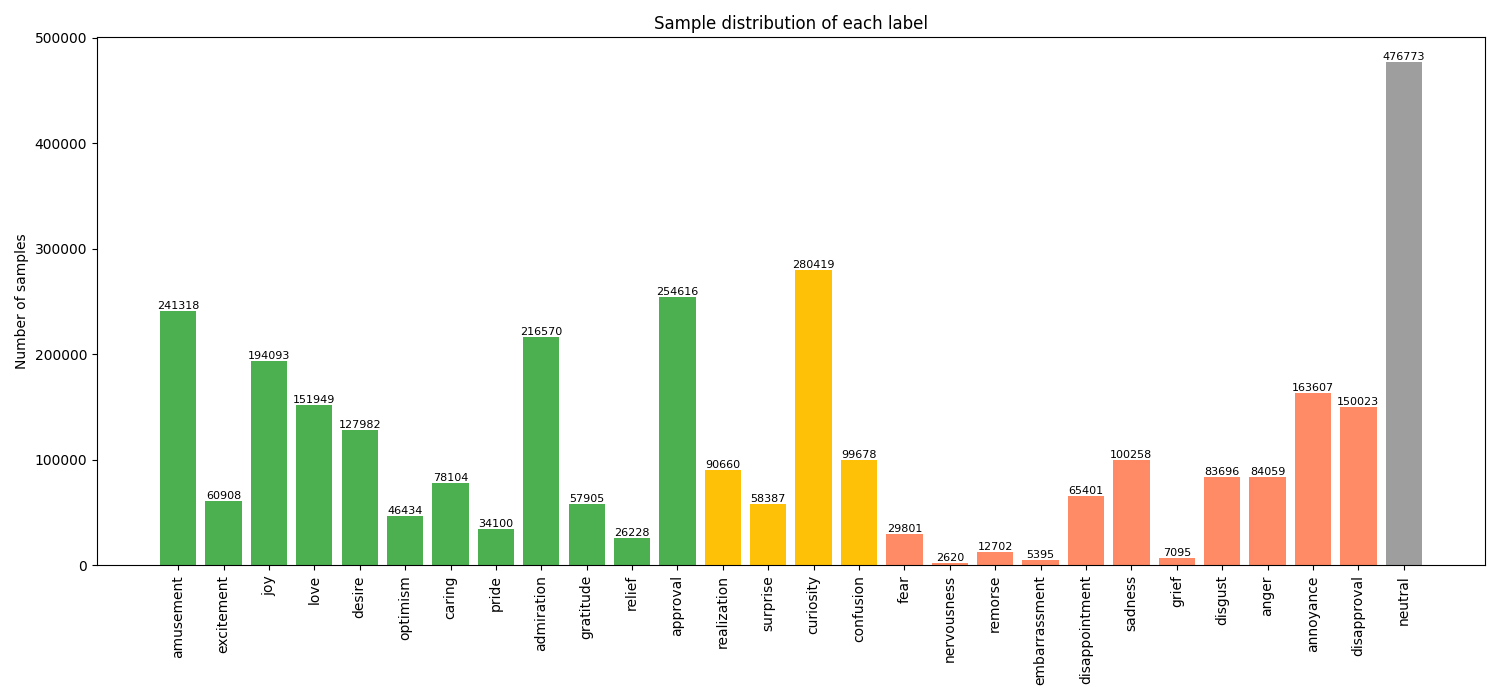
\includegraphics[width=0.8\textwidth]{Images/label_distribution.png}
    \caption{Phân phối dữ liệu theo đầu vào các nhóm cảm xúc: tích cực (xanh), tiêu cực (đỏ) và mập mờ (vàng).}
    \label{fig:bfdist}
    \vspace{0.1cm}
\end{figure}

\begin{figure}[htbp]
    \centering
    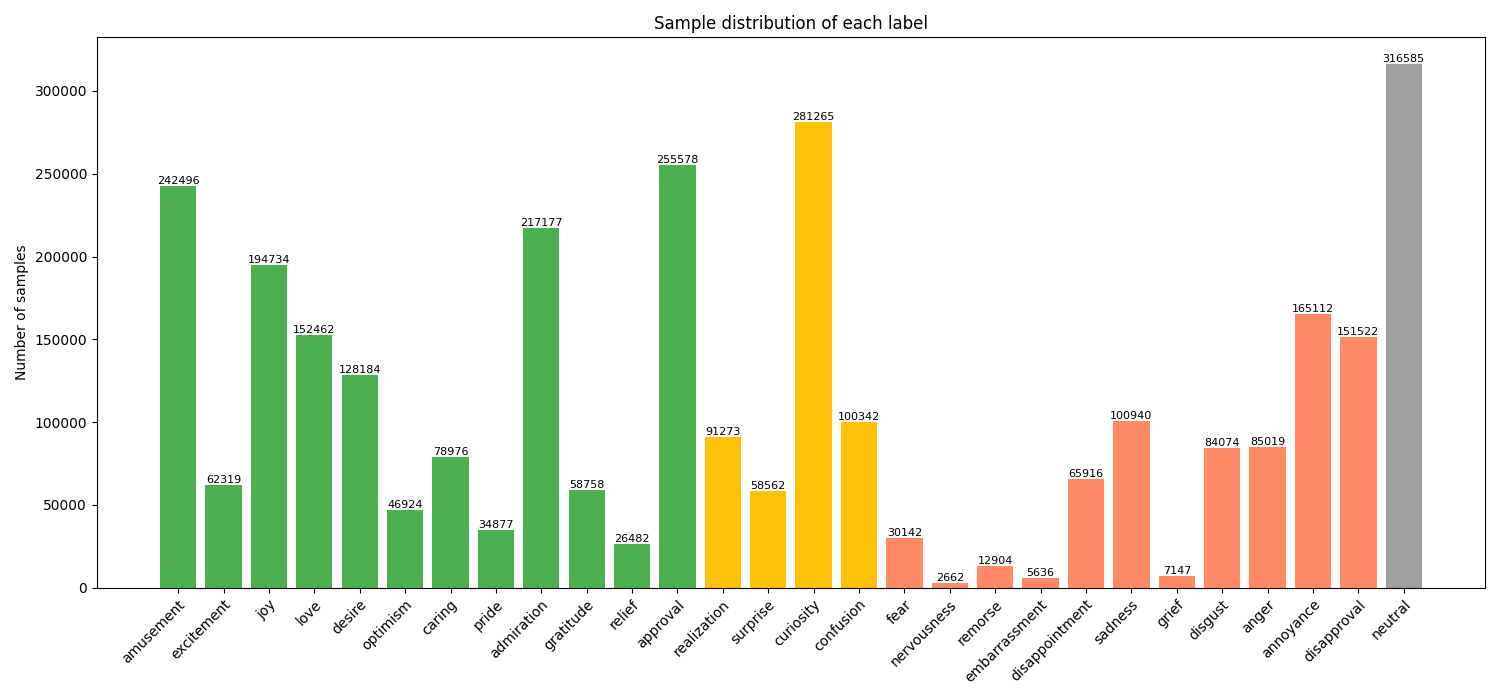
\includegraphics[width=0.8\textwidth]{Images/label_dist_after_unsampling.png}
    \caption{Phân phối dữ liệu theo các nhóm cảm xúc sau khi giảm mẫu (Unsampling). Tích cực (xanh), tiêu cực (đỏ) và mập mờ (vàng).}
    \label{fig:afdist}
    \vspace{0.1cm}
\end{figure}

\subsection{Xử lý mất cân bằng dữ liệu (Handling Imbalanced Data)}
Vì vẫn tồn tại sự mất cân bằng đáng kể giữa các nhóm cảm xúc tích cực và tiêu cực. Đặc biệt, các nhãn cảm xúc vi mô hiếm gặp (như sợ hãi - \texttt{fear}, lo lắng - \texttt{nervousness}, thương tiếc - \texttt{grief}, \dots) chiếm tỷ trọng rất nhỏ. Do đó, việc huấn luyện hoặc tinh chỉnh mô hình trực tiếp trên tập dữ liệu này mà không có biện pháp can thiệp sẽ dẫn đến hiệu suất thấp. Mô hình dễ rơi vào trạng thái cực đoan, khái quát hóa quá mức trên các nhãn đa số (tích cực) và bỏ qua các nhãn thiểu số (tiêu cực).

Để giải quyết vấn đề này, quá trình mô hình hóa cần phải áp dụng kết hợp phương pháp \textbf{Class-Balanced Loss (CB-Loss)} do \textcite{cui2019class} đề xuất và \textbf{Gradient Harmonized Mechanism Loss (GHM-Loss)} do \textcite{li2019gradient} đề xuất nhằm điều chuẩn (regularize) quá trình huấn luyện. Nhờ có sự tận dụng khả năng định hướng trọng số theo phân phối lớp của CB-Loss và khả năng điều tiết dựa trên độ khó thực tế của từng mẫu dữ liệu từ GHM-Loss. Sự cộng hưởng này sẽ giúp mô hình không bị áp đảo bởi các lớp có số lượng mẫu lớn, đồng thời tránh được hiện tượng quá khớp (overfitting) vào các mẫu nhiễu (outliers). Cụ thể, cơ sở toán học của phương pháp được biểu diễn như sau:

Giả sử một mẫu dữ liệu có nhãn thực (true label) là $y \in \{1, 2, \dots, C\}$ (với $C$ là số lượng nhãn) và xác suất dự đoán của mô hình cho lớp $y$ là $p_{y}$. Gọi $g$ là độ lớn gradient của mẫu dữ liệu đối với đầu ra của mô hình, được định nghĩa bằng $g = |p_{y} - 1|$.

\textbf{Class-Balanced Loss} được thiết kế để giải quyết bài toán mất cân bằng dữ liệu bằng cách sử dụng khái niệm \textit{số lượng mẫu hiệu dụng (effective number of samples)} nhằm tính toán trọng số cân bằng cho một lớp cụ thể $y$:

$$W_{y} = \frac{1 - \beta}{1 - \beta^{n_{y}}}$$

Trong đó:
\begin{itemize}[label=-]
    \item $n_{y}$ là số lượng mẫu của lớp $y$ trong toàn bộ tập dữ liệu huấn luyện.
    \item $\beta \in [0, 1)$ là một siêu tham số điều chỉnh (thông thường $\beta = 0.99$ hoặc $0.999$).
\end{itemize}

Khi đó, hàm mất mát CB-Loss áp dụng trên hàm \textbf{Cross-Entropy (CE)} tiêu chuẩn có dạng:

$$\mathcal{L}_{\text{CB}}(p_y) = -\frac{1 - \beta}{1 - \beta^{n_y}} \log(p_y)$$

\textbf{Gradient Harmonized Mechanism Loss (GHM-Loss)} được đề xuất nhằm điều chỉnh trọng số của mẫu dựa trên Mật độ Gradient (Gradient Density), giúp giảm thiểu ảnh hưởng của các mẫu quá dễ dự đoán hoặc các mẫu nhiễu cực khó. Hàm mật độ gradient của một giá trị $g$ được xác định bằng:

$$GD(g) = \frac{1}{R_{i}} \sum_{k=1}^{N} \delta(g_{k}, g)$$

Trong đó:
\begin{itemize}[label=-]
    \item $N$ là tổng số mẫu trong một batch huấn luyện (training batch).$g_{k}$ là độ lớn gradient của mẫu thứ $k$.
    \item $\delta(g_{k}, g)$ là hàm chỉ dấu, có giá trị bằng $1$ nếu $g_{k}$ nằm trong khoảng (bin) của $g$ và bằng $0$ trong trường hợp ngược lại.
    \item $R_{i}$ là độ rộng của khoảng chứa $g$.
\end{itemize}

Với hệ số điều hòa GHM được tính bằng nghịch đảo của mật độ $\hat{\beta}_{i}=\frac{N}{GD(g)}$, hàm mất mát GHM-Loss được định nghĩa như sau:

$$\mathcal{L}_{\text{GHM}} = \frac{1}{N} \sum_{i=1}^{N} \frac{-\log(p_{y, i})}{GD(g_{i})}$$

Để đồng thời tối ưu hóa cả hai khía cạnh — cân bằng số lượng mẫu hiệu dụng giữa các lớp và điều hòa độ khó của từng mẫu riêng lẻ — hàm mất mát hỗn hợp (Mixture Loss) được triển khai như sau:

$$\mathcal{L}_{\text{Mixture}} = W_y \cdot \mathcal{L}_{\text{GHM}}$$

\subsection{Lựa chọn mô hình thực nghiệm}

Do khung phương pháp được thiết kế tập trung vào các kiến trúc Transformer dạng Encoder, quy trình thực nghiệm giới hạn đánh giá trên các mô hình thuộc họ BERT. Dựa trên tiến trình phát triển của công nghệ xử lý ngôn ngữ tự nhiên, ba mô hình đại diện được lựa chọn bao gồm:
\begin{itemize}
    \item \textbf{mBERT} \parencite{devlin2019bert}: Được phát hành bởi Google cùng thời điểm với BERT. Đây là một trong những mô hình tiên phong của kỷ nguyên tiền huấn luyện đa ngôn ngữ, được huấn luyện đồng thời trên ngữ liệu Wikipedia của 104 ngôn ngữ khác nhau (bao gồm cả tiếng Việt).
    \item \textbf{PhoBERT} \parencite{nguyen2020phobert}: Mô hình đơn ngôn ngữ (Monolingual) dựa trên kiến trúc RoBERTa, được huấn luyện hoàn toàn bằng một kho ngữ liệu tiếng Việt quy mô lớn (30GB văn bản thô từ báo chí, văn học và mạng xã hội). Nhờ chiến lược phân mảnh từ (word segmentation) ở đầu vào (ví dụ: \texttt{học sinh} được nối thành \texttt{học\_sinh}), mô hình có khả năng nắm bắt trực tiếp các đặc trưng ngữ nghĩa ở cấp độ từ vựng trong tiếng Việt.
    \item \textbf{mModernBERT} \parencite{warner2025smarter}: Phiên bản đa ngôn ngữ của ModernBERT, đại diện cho kiến trúc đã được tối ưu hóa sâu sắc so với bản gốc của BERT. Mô hình này mở rộng độ dài ngữ cảnh lên tới 8192 token, tích hợp cơ chế Attention tăng tốc phần cứng, và thay thế cơ chế mã hóa vị trí tuyệt đối bằng Rotary Position Embedding (RoPE). Những cải tiến này giúp mô hình bắt giữ vị trí và khoảng cách của từ trong câu tốt hơn, từ đó gia tăng độ nhạy bén với các cấu trúc ngữ pháp lỏng lẻo đặc trưng của ngôn ngữ mạng xã hội.
\end{itemize}
